
\documentclass[a4paper,14pt]{extreport}
\usepackage[utf8]{inputenc}
\usepackage[T2A]{fontenc}
\usepackage[russian]{babel}
\usepackage{amssymb,amsfonts,amsmath}
\usepackage{multicol}
\usepackage{graphicx}
\usepackage{listings}
\usepackage{alltt}
\usepackage{verbatim}
\usepackage{listingsutf8}
\usepackage[
 left=25mm,
 top=20mm,
 right=10mm, 
 bottom=20mm, 
 nohead, 
 nofoot] {geometry}
\pagenumbering{arabic}

\parindent=0pt

\newcommand{\labtitle}{
 
}
\newcommand{\labnumber}{4}

\begin{document}
\title{Отчет по лабораторной работе \labnumber}
\author{Vladislav Tsisyk}
\thispagestyle{empty}
\begin{center}
\normalsize{Министерство образования и науки Российской Федерации}\\
\vspace{0.3cm}
\normalsize{Федеральное государственное бюджетное образовательное учреждение \\
высшего профессионального образования \\
«Алтайский государственный технический университет им. И.И. Ползунова»}\\*
\end{center}


\vspace{0.5cm}

\begin{flushleft} {
{\underline{Факультет Информационных Технологий}} \\
\vspace{0.2cm}
{Кафедра \underline{прикладной математики}} \\
\vspace{0.2cm}
}
\begin{tabular*}{\textwidth}{@{}l@{\extracolsep{\fill}}l}
~  &   Отчет защищен с оценкой \hrulefill \\
~ & Преподаватель \hrulefill\underline{\hspace{4cm}} Н.~Д.~Бубнова\\
~ & <<\underline{\hspace{0.8cm}}>> ~\underline{\hspace{3cm}} 2015 г.\\
\end{tabular*}

\end{flushleft}

\vspace{0.1cm}
\begin{center} {
\large{Отчет \\ по лабораторной работе №\labnumber} \\

\labtitle
}
\begin{center}
    I  семестр
 \end{center}
\vspace{0.4cm}

\linespread{0.7}{\Large{по дисциплине <<Введение в алгоритмы и основы технолог. разраб. пр.>>}}



\end{center}
\vspace{7cm}

\begin{center}

\begin{tabular*}{1.0\textwidth}{ll@{\extracolsep{\fill}}c}
Студент группы ПИ-41  & \underline{\hspace{6cm}}~В.~О.~Цисык & ~\\
Преподаватель \hfill & \underline{\hspace{6cm}}~Н.~Д.~Бубнова & ~ \\
\end{tabular*}
\end{center}

\vspace{\fill}

\begin{center}
\Large{БАРНАУЛ 2015}
\end{center}
\newpage

\textbf{Задание:}\\
		Вставить вместо элемента с заданным значением новый список.
\subsection*{Описание алгоритма:}
Программа начинает свое выполнение с того, что запрашивает у пользователя файл с исходными данными.
Если файл с заданным именем существует, то создается пустой список, в который по очереди записываются в конец исходные данные.
Аналогично поступаем со вторым списком. Запрашиваем у пользователя позицию для вставки.

Списки и позиция для вставки передаются в функцию list\_insert().\\ 

Если позиция для вставки списка меньше нуля или список, в который необходимо сделать встаку пуст, то возвращается пустой список. 
Просматриваем список до тех пор, пока не дойдем до нужной позиции в списке. Иначе возвращаем пустой список. 

Нужная позиция в списке существует, теперь необходимо вставить список в список. 
Обозначим список, в который вставляем буквой A, а список для вставки - буквой B.

Сначала мы присоединяем к концу списка B те элементы списка A, что стоят после выбранной позиции. 
В начало полученного списка вставить те элементы списка А, которые предшествуют заменяемому новым списком элементу.
После устанавливаем указатели на первый и последний элемент в списке. Возвращаем список в вызывающую функцию. 


\subsection*{Код программы:}
\small
\begin{verbatim}
/* list.h */

 struct Node{
	int number;
	struct Node *next;
	struct Node *previous;
};

struct List{
	struct Node *head;
	struct Node *tail;
};

struct List *list_init(void);
void list_append(struct List *test, int number);
struct List *list_LIS(struct List *test);
struct List *list_insert(struct List *test, struct List *ap, int pos);
void list_push(struct List *test, int number);
/* list.c */
#include <stdlib.h>
#include <assert.h>
#include <stdio.h>
#include "list.h"

/* Создаем новый список */
struct List *list_init(void)
{
	struct List* theList = malloc(sizeof(struct List));
	assert(theList != NULL);

	theList->head = NULL;
	theList->tail = NULL;
	return theList;
}
/* 	Функция вставки списка в список, начиная с определенной позиции.
	Если Вставляемый список, список, в который нужно вставить, пусты
  	или позиции для вставки превосходят/меньше размера списка, 
	то возвращается пустой список
 */
struct List *list_insert(struct List *test, struct List *toinsert, int pos)
{
	
	int i;
	struct List *ap = NULL;
	struct Node *tmp= test->head;
	ap = list_init();
	if(test->head == NULL || pos < 0)
		return test;

	for(i = 0; i < pos; i++){
		if(tmp->next == NULL){
			return ap;
		}
		tmp = tmp->next;
	}
	/* Подцепляем "конец" одного списка */
	if(toinsert->head == NULL){
		if(tmp->next !=NULL)
			tmp->next->previous = tmp->previous;
		else
			test->tail = tmp->previous;
		if(tmp->previous != NULL)
			tmp->previous->next = tmp->next;
		else 
			test->head = tmp->next;
		return test;
	}
	ap = toinsert;
	ap->tail->next = tmp->next;

	if(tmp->next != NULL)
		tmp->next->previous = ap->tail;
	/* подцепляем "начало" списка */
	if(tmp->previous != NULL){
		tmp = tmp->previous;
		tmp->next = ap->head;
		ap->head->previous = tmp;
	}else{
		ap->head->previous = NULL;
	}

	/* устанавливаем указатели на начало и конец списка*/
	while(ap->head->previous != NULL)
		ap->head = ap->head->previous;

	while(ap->tail->next != NULL)
		ap->tail = ap->tail->next;

	return ap;
	
}
/* Добавляем в конец списка */
void list_append(struct List *test, int number)
{
	struct Node *newNode = malloc(sizeof(struct Node));
	assert(newNode != NULL);
	newNode->number = number;
	newNode->next = NULL;
	newNode->previous = test->tail;
	if(test->head == NULL)
		test->head = test->tail = newNode;
	else{
		test->tail->next = newNode;
		test->tail = newNode;
	}
}

/* Добавляем в начало списка */
void list_push(struct List *test, int number)
{
	struct Node *newNode = malloc(sizeof(struct Node));
	newNode->number = number;
	newNode->next = NULL;	
	if(test->head == NULL)
		test->head = test->tail = newNode;
	else{
		newNode->next = test->head;
		test->head = newNode;
	}
}

/* Обрабатываем список  */
struct List *list_LIS(struct List *test)
{
	int *prev = NULL;
	int *len = NULL;
	struct Node *tmp = test->head;
	struct Node *first = NULL;
	struct List *answer = NULL;
	answer = list_init();
	int i,j, n;
	int pos, length;
	length = i =  0;

	/* пуст ли список? */

	if(tmp == NULL)
		return answer;	
	while(tmp != NULL){

		/* выделить память под очередные элементы массива*/
		prev = realloc(prev, (++length) * sizeof(int));
		len = realloc(len, (++length) * sizeof(int));
		/* запомнить позицию головы */
		first = test->head;
		prev[i] = -1;
		len[i] = j = 0;

		/* находим количество элементов меньше определенного */
		while(first != tmp){
			if(first->number <= tmp->number &&
			len[j] + 1 > len[i]){
				len[i] = len[j] + 1; 
				prev[i] = j;
			}
			first = first->next;
			j++;
		}
		/* printf("%d --- %d --- %d\n", len[i], tmp->number, prev[i]);*/
		tmp = tmp->next;
		i++;
	}
	/* находим самую длинную последовательность чисел... */
	n = length;
	pos = 0;
	length = len[0];
	for(i = 0; i < n; i++)
		if(len[i] > length){
			pos = i;
			length = len[i];
		}

	tmp = test->head;
	i = 0;
	/* ...и пихаем ее в список */
	while(pos != -1){
		for(i = 0; i < pos; i++)
			tmp = tmp->next;
		list_push(answer, tmp->number);
		pos = prev[pos];
		tmp = test->head;
	}

	return answer;
}
/* Вставить вместо элемента с заданным значением новый список */
#include <stdio.h>
#include "list.h"
#define LINELENGTH 1024
int main()
{

	FILE *fp;
    char line[LINELENGTH];
    char *p;
	int c, n;
	char anw;
	struct List *test = NULL;
	struct List *answer = NULL;
	struct List *combined = NULL;
	test = list_init();
	answer = list_init();
	combined = list_init();
   
   	printf("введите имя файла:");
    scanf("%s", line);
    if((fp = fopen(line,"r")) == NULL){
        fprintf(stderr, "Нет такого файла\n");
        return 1;
    }
    /* читаем строку за строкой */
	p = line;
    while(fgets (line, LINELENGTH, fp)){
         while(sscanf(p, "  %d%n", &c, &n) == 1 ){
			list_append(test, c);
             p +=n;
        }
    }

	fclose(fp);
	printf("введите имя файла:");
    scanf("%s", line);
    if((fp = fopen(line,"r")) == NULL){
        fprintf(stderr, "Нет такого файла\n");
        return 1;
    }
    /* читаем строку за строкой */
	p = line;
    while(fgets (line, LINELENGTH, fp)){
         while(sscanf(p, "  %d%n", &c, &n) == 1 ){
			list_append(answer, c);
             p +=n;
        }
    }
	fclose(fp);
	printf("введите позицию для вставки:");
		scanf("%d", &c);
	combined = list_insert(test,answer, c);
/*
	while(combined->head != NULL){
		printf("%d ",combined->head->number);	
		combined->head = combined->head->next;
	}
	printf("\n");
	while(combined->tail != NULL){
		printf("%d ",combined->tail->number);	
		combined->tail = combined->tail->previous;
	}
	printf("\n");

*/

	while ((anw = getchar())!= '\n' && anw != EOF);
	printf("Сохранить в файл? [y/n]:");
	scanf("%c", &anw);
	switch (anw){
    	case 'y': case 'Y': 
    	fp = fopen("output.txt", "a");
    	fprintf(fp, "------------------------\n");
		while(combined->head != NULL){
			fprintf(fp, "%d ", combined->head->number);
			combined->head = combined->head->next;
		}
    	fprintf(fp,"\n");
    	fclose(fp);
    	break;
	}

	return 0;
}
\end{verbatim}
\normalsize
\subsection*{Результаты тестирования:}
\begin{center}
	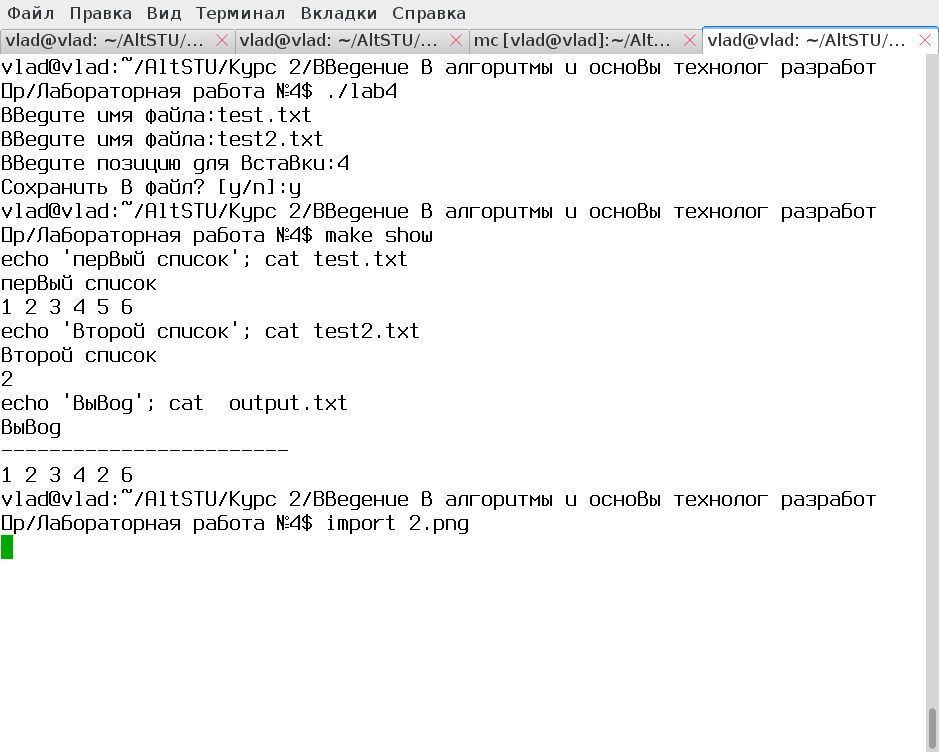
\includegraphics[scale = 0.5]{2.png}
\end{center}

\end{document}
